%%
%% This is file `./samples/longsample.tex',
%% generated with the docstrip utility.
%%
%% The original source files were:
%%
%% apa6.dtx  (with options: `longsample')
%% ----------------------------------------------------------------------
%% 
%% apa6 - A LaTeX class for formatting documents in compliance with the
%% American Psychological Association's Publication Manual, 6th edition
%% 
%% Copyright (C) 2011-2016 by Brian D. Beitzel <brian at beitzel.com>
%% 
%% This work may be distributed and/or modified under the
%% conditions of the LaTeX Project Public License (LPPL), either
%% version 1.3c of this license or (at your option) any later
%% version.  The latest version of this license is in the file:
%% 
%% http://www.latex-project.org/lppl.txt
%% 
%% Users may freely modify these files without permission, as long as the
%% copyright line and this statement are maintained intact.
%% 
%% This work is not endorsed by, affiliated with, or probably even known
%% by, the American Psychological Association.
%% 
%% ----------------------------------------------------------------------
%% 
\documentclass[man]{apa6}

\usepackage{lipsum}

\usepackage[american]{babel}

\usepackage{csquotes}
\usepackage[style=apa,sortcites=true,sorting=nyt,backend=biber]{biblatex}
\DeclareLanguageMapping{american}{american-apa}
\addbibresource{bibliography.bib}

\title{Sample APA-Style Document Using the \textsf{apa6} Package}
\shorttitle{Sample Document}

\author{Brian D. Beitzel}
\affiliation{SUNY Oneonta}

\leftheader{Beitzel}

\abstract{\lipsum[1]}

\keywords{APA style, demonstration}

\authornote{Brian D. Beitzel, Department of Educational Psychology,
  Counseling and Special Education, SUNY Oneonta.

  Correspondence concerning this article should be addressed to Brian
  D. Beitzel, Department of Educational Psychology, Counseling and
  Special Education, SUNY Oneonta, 129 Fitzelle Hall, Oneonta, NY
  13820.  E-mail: beitzebd@oneonta.edu}

\begin{document}
\maketitle
\lipsum[2]

\Textcite{vonDavier2011} said this,
too \parencite{vonDavier2011,Lassen2006}.  Further evidence comes from
other sources \parencite{Shotton1989,Lassen2006}.  \lipsum[3]

\section{Method}
\subsection{Participants}
\lipsum[4]

\subsection{Materials}
\lipsum[5]

\subsection{Design}
\lipsum[6]

\subsection{Procedure}
\lipsum[7]

\subsubsection{Instrument \#1}
\lipsum[8]

\paragraph{Reliability}
\lipsum[9]

\subparagraph{Inter-rater reliability}
\lipsum[10]

\subparagraph{Test-retest reliability}
\lipsum[11]

\paragraph{Validity}
\lipsum[12]

\subparagraph{Face validity}
\lipsum[13]

\subparagraph{Construct validity}
\lipsum[14]

\section{Results}
Table~\ref{tab:BasicTable} summarizes the data. \lipsum[15]

\begin{table}
  \caption{Sample Basic Table}
  \label{tab:BasicTable}
  \begin{tabular}{@{}llr@{}}         \toprule
  \multicolumn{2}{c}{Item}        \\ \cmidrule(r){1-2}
  Animal    & Description & Price \\ \midrule
  Gnat      & per gram    & 13.65 \\
            & each        &  0.01 \\
  Gnu       & stuffed     & 92.50 \\
  Emu       & stuffed     & 33.33 \\
  Armadillo & frozen      &  8.99 \\ \bottomrule
  \end{tabular}
\end{table}

\begin{figure}
    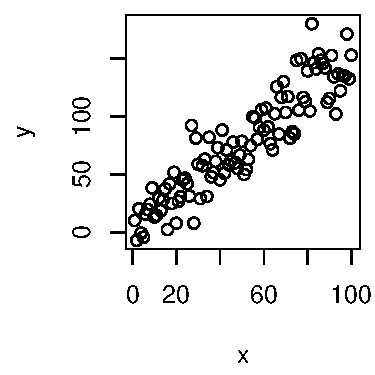
\includegraphics[bb=0in 0in 2.5in 2.5in, height=2.5in, width=2.5in]{Figure1.pdf}
    \caption{This is my first figure caption.}
    \label{fig:Figure1}
\end{figure}

Figure~\ref{fig:Figure1} shows this trend. \lipsum[16]

\section{Discussion}
\lipsum[17]

\lipsum[18]

\lipsum[19]

\printbibliography

\appendix

\section{Instrument}
\label{app:instrument}

As shown in Figure~\ref{fig:Figure2}, these results are impressive. \lipsum[20]

\begin{figure}
    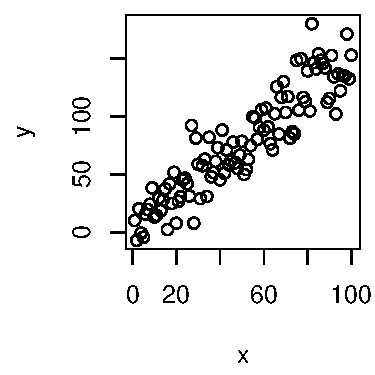
\includegraphics[bb=0in 0in 2.5in 2.5in, height=2.5in, width=2.5in]{Figure1.pdf}
    \caption{This is my second figure caption.}
    \label{fig:Figure2}
\end{figure}

\lipsum[21]
\section{Pilot Data}
\label{app:surveydata}

The detailed results are shown in Table~\ref{tab:DeckedTable}. \lipsum[22]

\begin{table}
  \begin{threeparttable}
    \caption{A More Complex Decked Table}
    \label{tab:DeckedTable}
    \begin{tabular}{@{}lrrr@{}}         \toprule
    Distribution type  & \multicolumn{2}{l}{Percentage of} & Total number   \\
                       & \multicolumn{2}{l}{targets with}  & of trials per  \\
                       & \multicolumn{2}{l}{segment in}    & participant    \\ \cmidrule(r){2-3}
                                    &  Onset  &  Coda            &          \\ \midrule
    Categorical -- onset\tabfnm{a}  &    100  &     0            &  196     \\
    Probabilistic                   &     80  &    20\tabfnm{*}  &  200     \\
    Categorical -- coda\tabfnm{b}   &      0  &   100\tabfnm{*}  &  196     \\ \midrule
    \end{tabular}
    \begin{tablenotes}[para,flushleft]
        {\small
            \textit{Note.} All data are approximate.

            \tabfnt{a}Categorical may be onset.
            \tabfnt{b}Categorical may also be coda.

            \tabfnt{*}\textit{p} < .05.
            \tabfnt{**}\textit{p} < .01.
         }
    \end{tablenotes}
  \end{threeparttable}
\end{table}

\lipsum[23]

\end{document}

%% 
%% Copyright (C) 2011-2016 by Brian D. Beitzel <brian at beitzel.com>
%% 
%% This work may be distributed and/or modified under the
%% conditions of the LaTeX Project Public License (LPPL), either
%% version 1.3c of this license or (at your option) any later
%% version.  The latest version of this license is in the file:
%% 
%% http://www.latex-project.org/lppl.txt
%% 
%% Users may freely modify these files without permission, as long as the
%% copyright line and this statement are maintained intact.
%% 
%% This work is not endorsed by, affiliated with, or probably even known
%% by, the American Psychological Association.
%% 
%% 
%% This work is "maintained" (as per LPPL maintenance status) by
%% Brian D. Beitzel.
%% 
%% This work consists of the file  apa6.dtx
%% and the derived files           apa6.ins,
%%                                 apa6.cls,
%%                                 apa6.pdf,
%%                                 README,
%%                                 APAamerican.txt,
%%                                 APAbritish.txt,
%%                                 APAdutch.txt,
%%                                 APAenglish.txt,
%%                                 APAgerman.txt,
%%                                 APAngerman.txt,
%%                                 APAgreek.txt,
%%                                 APAczech.txt,
%%                                 APAturkish.txt,
%%                                 APAendfloat.cfg,
%%                                 apa6.ptex,
%%                                 TeX2WordForapa6.bas,
%%                                 Figure1.pdf,
%%                                 shortsample.tex,
%%                                 longsample.tex, and
%%                                 bibliography.bib.
%% 
%%
%% End of file `./samples/longsample.tex'.
